
\newpage
{\bfseries МРНТИ 65.33.29}

\sectionwithauthors{Д.А. Шаймерденова, А.М. Омаралиева, Б.К. Тарабаев, Л.Т. Сарбасова, С.С. Ануарбекова, \textsuperscript{1}Д.Б.
Искакова, А.А. Шаймерденов ,Д.А. Тастанов}{ПРОИЗВОДСТВО ОБОГАЩЕННЫХ МАКАРОННЫХ ИЗДЕЛИЙ КОМПЛЕКСОМ
НАНОКАРБОКСИЛАТОВ И ТОНКОДИСПЕРСНЫМ ПОРОШКОМ ЗЕРНОВЫХ КУЛЬТУР}
\begin{center}

{\bfseries \textsuperscript{1}Д.А. Шаймерденова\textsuperscript{🖂},
\textsuperscript{2}А.М. Омаралиева, \textsuperscript{3}Б.К. Тарабаев,
\textsuperscript{1}Л.Т. Сарбасова,}

{\bfseries \textsuperscript{1}С.С. Ануарбекова, \textsuperscript{1}Д.Б.
Искакова, \textsuperscript{1}А.А. Шаймерденов , \textsuperscript{1}Д.А.
Тастанов}

\textsuperscript{1}ТОО «Научно-производственное предприятие «Инноватор»,
Астана, Казахстан,

\textsuperscript{2} Казахский университет технологии и бизнеса
им.К.Кулажанова, Астана, Казахстан,

\textsuperscript{3} Казахский агротехнический исследовательский
университет им. С. Сейфуллина, Астана, Казахстан
\end{center}

\textsuperscript{🖂}Коррреспондент-автор: e-mail: darigash@mail.ru\vspace{0.5cm}

Объект исследований -- макаронные изделия, обогащённые тонкодисперсной
мукой из гречихи и чечевицы, и комплексом нанонокарбоксилатов.

По данным аналитиков, потребление макаронных изделий в Казахстане ---
одно из самых высоких в мире, Казахстан уступает в этом только Италии.
За январь -- декабрь 2022 года производство макарон составило 166,1 тыс.
тонн, что на 4\% больше, чем в 2021 году {[}1{]}.

Учитывая, что макаронные изделия популярны и потребляются в большом
количестве, имеется возможность реально и эффективно проводить
профилактику различных видов заболеваний с помощью выпуска изделий с
использованием обогащающих комплексов микроэлементов и витаминов. Тем
более, что основным сырьем для производства макарон является
«обедненная» пшеничная мука высшего сорта. В то же время, продукты
питания серьёзно дорожают, что неизбежно сказывается на
продовольственной безопасности республики {[}1{]}.

В этой связи необходима разработка отечественных технологий производства
обогащённых макаронных изделий, что позволит повысить их
конкурентоспособность за счет снижения себестоимости.

В рамках исследований получены макаронные изделия, обогащенные наиболее
ценной по содержанию белка и клетчатки чечевичным и гречневым
тонкодисперсным порошком в количестве 10\%. Для обогащения макаронных
изделий микро- и макроэлементами произведен подбор и расчет рецептур
нанокарбоксилатов с установлением их количества, исходя из норм
потребления человека. По химическому и микроэлементному составу
определены наиболее полноценные добавки.

Результаты исследований позволили установить, что потребительские
свойства макаронных изделий, обогащенных тонкодисперсным порошком из
гречихи, соответствуют нормативным показателям. Комплекс
нанокарбоксилатов не повлиял на потребительские свойства макарон, но
значительно увеличил содержание магия и цинка.

{\bfseries Ключевые слова:} макароны, тонкодисперсный порошок,
нанокарбоксилаты, микроэлементы, чечевичная мука, гречневая мука.

\sectionheading{НАНОКАРБОКСИЛАТТАР КЕШЕНІМЕН ЖӘНЕ ДӘНДІ ДАҚЫЛДАРДЫҢ ЖҰҚА
ДИСПЕРСТІ ҰНТАҒЫМЕН БАЙЫТЫЛҒАН МАКАРОН ӨНІМДЕРІН ӨНДІРУІ}
\begin{center}

{\bfseries \textsuperscript{1}Д.А. Шаймерденова\textsuperscript{🖂},
\textsuperscript{2}А.М. Омаралиева, \textsuperscript{3}Б.К. Тарабаев,
\textsuperscript{1}Л.Т.Сарбасова,}

{\bfseries \textsuperscript{1}С.С. Ануарбекова, \textsuperscript{1}Д.Б.
Искакова, \textsuperscript{1}А.А. Шаймерденов , \textsuperscript{1}Д.А.
Тастанов}

\textsuperscript{1}«Инноватор» Ғылыми-өндірістік кәсіпорны» ЖШС, Астана,
Қазақстан,

\textsuperscript{2} Қ.Құлажанов атындағы Қазақ технология және бизнес
университеті, Астана, Қазақстан,

\textsuperscript{3}С.Сейфуллин атындағы Қазақ агротехникалық зерттеу
университеті, Астана, Қазақстан,

e-mail: darigash@mail.ru
\end{center}

Зерттеу нысаны-қарақұмық пен жасымық ұнымен және нанокарбоксилаттар
кешенімен байытылған макарон өнімдері.

Сарапшылардың пікірінше, Қазақстанда макарон өнімдерін тұтыну әлемдегі
ең жоғары көрсеткіштердің бірі болып табылады, Қазақстан бұл жағынан
Италиядан кейін екінші орында. 2022 жылдың қаңтар -- желтоқсан айларында
макарон өндірісі 166,1 мың тоннаны құрады, бұл 2021 жылмен салыстырғанда
4\% - ға өсті {[}1{]}

Макарон өнімдері танымал және көп мөлшерде тұтынылатындығын ескере
отырып, микроэлементтер мен дәрумендерді байытатын кешендерді қолдана
отырып, өнімдерді шығару арқылы әртүрлі аурулардың алдын-алуды нақты
және тиімді жүргізуге болады. Сонымен қатар, макарон өндірісінің негізгі
шикізаты-жоғары сортты "сарқылған" бидай ұны. Сонымен қатар, Азық-түлік
қатты бағаланады, бұл сөзсіз республиканың азық-түлік қауіпсіздігіне
әсер етеді {[}1{]}.

Осыған байланысты байытылған макарон өнімдерін өндірудің отандық
технологияларын әзірлеу қажет, бұл өзіндік құнын төмендету есебінен
олардың бәсекеге қабілеттілігін арттыруға мүмкіндік береді.

Зерттеулер аясында 10\% мөлшерінде жасымық және қарақұмық жұқа дисперсті
ұнтағымен ақуыз және талшық құрамы бойынша ең құнды байытылған макарон
өнімдері алынды. Макарон өнімдерін микро және макроэлементтермен байыту
үшін нанокарбоксилаттардың рецептураларын таңдау және есептеу адамның
тұтыну нормаларына сүйене отырып, олардың санын белгілеу арқылы жүзеге
асырылады. Химиялық және микроэлементтік құрамы бойынша ең толыққанды
қоспалар анықталды.

Зерттеу нәтижелері қарақұмық ұнтағымен байытылған макарон өнімдерінің
тұтынушылық қасиеттері нормативтік көрсеткіштерге сәйкес келетіндігін
анықтады. Нанокарбоксилат кешені макаронның тұтынушылық қасиеттеріне
әсер етпеді, бірақ оның құрамын едәуір арттырды сиқыр және мырыш.

{\bfseries Түйін сөздер:} макарон, жұқа дисперсті ұнтак,
нанокарбоксилаттар, микроэлементтер, жасымық ұны, қарақұмық ұны.

\sectionheading{PRODUCTION OF ENRICHED PASTA PRODUCTS WITH A COMPLEX OF
NANOCARBOXYLATES AND FINE-DISPERSED CEREAL FLOUR}
\begin{center}

{\bfseries \textsuperscript{1}D.A. Shaimerdenova\textsuperscript{🖂},
\textsuperscript{2}A.M. Omaralieva, \textsuperscript{3}B.K. Tarabaev,
\textsuperscript{1}L.T. Sarbasova,\\
\textsuperscript{1}S.S. Anuarbekova, \textsuperscript{1}D.B. Iskakova,
\textsuperscript{1}A.A. Shaimerdenov, \textsuperscript{1}D.A. Tastanov}

\textsuperscript{1}«Research and Production Enterprise «Innovator» LLP,
Astana,

\textsuperscript{2}K.Kulazhanov Kazakh University of Technology and
Business, Astana, Kazakhstan,

\textsuperscript{3}Kazakh Agrotechnical Research University named after
S. Seifullin, Astana, Kazakhstan,

e-mail : darigash@mail.ru
\end{center}

The object of research is pasta enriched with fine flour from buckwheat
and lentils, and a complex of nanocarboxylates.

According to analysts, the consumption of pasta in Kazakhstan is one of
the highest in the world, Kazakhstan is second only to Italy in this. In
January -- December 2022, pasta production amounted to 166.1 thousand
tons, which is 4\% more than in 2021 {[}1{]}

Considering that pasta is popular and consumed in large quantities, it
is possible to really and effectively prevent various types of diseases
by producing products using enriching complexes of trace elements and
vitamins. Moreover, the main raw material for the production of pasta is
"depleted" wheat flour of the highest grade. At the same time, food is
seriously becoming more expensive, which inevitably affects the food
security of the republic {[}1{]}.

In this regard, it is necessary to develop domestic technologies for the
production of enriched pasta, which will increase their competitiveness
by reducing the cost.

As part of the research, the most valuable fortified pasta in terms of
protein and fiber content was obtained with a fine-dispersed powder of
lentils and buckwheat in an amount of 10\%. The selection and
calculation of the formulations of nanocarboxylates for the enrichment
of pasta with micro and Macroelements is carried out by establishing
their number, based on the norms of human consumption. The most complete
additives in terms of chemical and microelement composition were
identified.

The results of the study found that the consumer properties of pasta
enriched with buckwheat powder correspond to regulatory indicators. The
nanocarboxylate complex did not affect the consumer properties of pasta,
but significantly increased the content of maggot and zinc.

{\bfseries Key words:} pasta, fine powder, nanocarboxylates, trace
elements, lentil flour, buckwheat flour.

{\bfseries Введение.} Макаронные изделия --- популярный во всем мире
продукт питания, известный простотой приготовления, хорошей
стабильностью при хранении, низкой стоимостью, простотой приготовления и
низким гликемическим индексом (ГИ). Макаронные изделия состоят в
основном из углеводов (70--76\%), белков (\textasciitilde10--14\%),
липидов (\textasciitilde1,8\%), пищевых волокон (\textasciitilde2,9\%) и
небольшого количества минералов и витаминов, Углеводы же в пищевых
продуктах являются важным источником энергии для человека {[}2{]}.
Однако, в макаронах мало пищевых волокон, витаминов, незаменимых
аминокислот и минералов {[}2{]}, т.к. при помоле для приготовления
макаронной муки происходит потеря этих компонентов. Макаронные изделия
можно считать хорошим средством для включения биологически активных
ингредиентов (белков, фитохимических веществ, минералов, витаминов и т.
д.), как это признано Всемирной организацией здравоохранения и
Управлением по санитарному надзору за качеством пищевых продуктов и
медикаментов США, поскольку в некоторых ситуациях до 10--15\% не-
традиционных ингредиентов могут быть добавлены без существенной потери
качества макаронных изделий в зависимости от используемого ингредиента и
технологии обработки макаронных изделий {[}3,4{]}.

Однако, польза от добавленного ингредиента, которую предполагается
обеспечить, может быть ограничена таким уровнем включения. При
разработке пищевых продуктов с биологически активными соединениями
получаемые продукты часто имеют технологические недостатки,
нежелательный внешний вид и органолептические свойства, что делает их
менее привлекательными для потребителей или просто нерентабельными в
производстве.

Основным сырьем, применяемым в макаронном производстве, является
пшеничная мука. Действующий в Казахстане нормативный документ {[}5{]}
предусматривает использование в качестве основного сырья макаронного
производства пшеничной муки высшего или I сортов. Лучшим сырьем для
макарон является специальная макаронная мука из твердой или
высокостекловидной мягкой пшеницы. Из такой муки получаются изделия
лучшего качества, имеющие янтарно-желтый или соломенно-желтый цвет.

Мука, используемая в макаронном производстве, не должна содержать в
значительных количествах свободные аминокислоты, редуцирующие сахара и
активную полифенолоксидазу (тирозиназу), вызывающую потемнение теста и
ухудшение качества готовых изделий. Вода является составной частью
макаронного теста. Она обусловливает биохимические и физико-химические
свойства теста. Используют водопроводную питьевую воду, которая должна
быть умеренно жесткой и отвечать требованиям нормативных документов на
питьевую воду {[}6{]}.

За последние два десятилетия было проведено много исследований по
повышению питательной ценности макаронных изделий за счет включения
нетрадиционных ингредиентов из-за спроса потребителей, заботящихся о
своем здоровье, на функциональные продукты {[}7,8{]}. Эти ингредиенты
могут влиять на технологические свойства макаронных изделий, но их
воздействие на здоровье не всегда измеряется, а скорее предполагается
{[}9{]}.

Так, в последнее время макаронные фабрики выпускают макаронные изделия,
при производстве которых могут применяться такие добавки, как
томат-пасты, шпинат, щавель, морковный сок. Не менее ценными являются
макаронные изделия, обогащенные минеральными веществами и с повышенным
содержанием пищевых волокон.

Однако, ассортиментный ряд макаронных изделий функциональной
направленности в настоящее время не так обширен. В виду плохой
экологической обстановки в мире, а также малоподвижного образа жизни
люди страдают от нехватки разного рода витаминов и полезных веществ.
Именно поэтому возник острый вопрос в обогащении продуктов повседневного
питания человека витаминами, минеральными и прочими полезными веществами
{[}10{]}.

В последнее время широко применяются для обогащения макаронных изделий
порошкообразные растительные источники, неоспоримым преимуществом
которых является высокая концентрация биологически активных веществ,
т.к. их масса меньше массы исходного сырья в 6-8 раз, имеется
возможность использования при производстве мучных изделий с низкой
влажностью, ввиду этого - длительный срок хранения и хорошая
транспортабельность {[}11{]}.

Ввиду этого, применение тонкодисперсных растительных порошков из
зерновых культур в качестве обогатителей и улучшителей макаронных
изделий представляет значительный интерес.

Тонкодисперсный порошок из зерна зерновых и бобовых культур --- это
цельнозерновой продукт, получаемый в результате технологической
обработки зерна, т.е. измельчении.

Главным вопросом, требующим решения в настоящее время, является изучение
возможности расширения видов муки из зерновых культур и нормы внесения,
которые позволят как повысить пищевую ценность, так и сохранить высокие
потребительские качества макаронных изделий.

Анализ литературы показывает, что среднесуточное потребление с пищей
каждого микронутриента, необходимого для поддержания нормальной
физиологической деятельности человека, измеряется в миллиграммах или в
меньших количествах и отличаются от макроэлементов (углеводов, жиров и
белков) и макроминералов (кальция, магния и фосфора).

Диетическая потребность человека в любом микронутриенте определяется
многими факторами, включая его биодоступность, количество, необходимое
для поддержания его нормальных физиологических функций и прочих факторов
{[}12{]}.

В то же время, по мнению экспертов, недостаток макро- и микроэлементов
приводит к значительным проблемам со здоровьем. В связи с этим возникает
жизненно-необходимая потребность в искусственном обогащении рациона ими
для обеспечения современного человека необходимым набором минеральных
веществ.

Так, например, на сегодня большинство жителей США, европейских стран,
Японии и все увеличивающаяся часть населения менее развитых стран
вынуждены регулярно употреблять дополнительные количества питательных
веществ. По данным американских ученых-диетологов, среднестатистический
рацион современного американца обеспечивает лишь 50--60 \%
рекомендованной суточной потребности в магнии (дефицит магния отмечен у
75--85 \% обследованных жителей США), лишь на 50 \% -- меди, селена,
кальция, около 70 и 90 \% человек недополучают с пищевыми продуктами
цинка и хрома {[}13{]}.

Дефицит микроэлементов приводит к негативным последствиям для здоровья.
Так, анализ научных данных о некоторых наиболее важных микро- и
макроэлементах и их воздействия на организм человека, показало
следующее.

Недостаток цинка вызывает заболевания центральной нервной,
желудочно-кишечной, иммунной, эпидермальной, репродуктивной и костной
систем, может повысить восприимчивость к болезням и инфекциям, увеличить
время восстановления или, в некоторых случаях, ухудшить восстановление,
снизить умственную работоспособность и увеличить последствия осложнений.
Распространенность дефицита цинка в странах Африки и Южной Азии
варьируется от 15 до 50\% {[}14{]}. По данным других исследователей,
дефицит цинка затрагивает более половины населения мира {[}15{]}.
Казахстан, относясь к странам с невысоким уровнем дохода населения,
также подвержен риску дефицита цинка в рационе питания населения.

Дефицит селена связан с сердечно-сосудистыми заболеваниями, бесплодием,
миодегенеративными заболеваниями и снижением когнитивных функций. В
настоящее время изучается роль селена в лечении рака. По данным
китайских ученых, результаты 8-летнего наблюдения показали снижение
заболеваемости первичным раком печени на 35,1\% у пациентов с
добавлением селенизированной поваренной соли по сравнению с населением,
не получавшим такой добавки {[}16-17{]}. Дефицит селена затрагивает от
500 млн. до 1 млрд. человек во всем мире из-за недостаточного его
потребления {[}18{]}.

Магний является четвертым наиболее распространенным катионом в организме
и вторым наиболее распространенным внутриклеточным катионом после калия
{[}19{]}, участвует в синтезе белков, нуклеиновых кислот, обладает
стабилизирующим действием для мембран, необходим для поддержания
гомеостаза кальция, калия и натрия. Недостаток магния приводит к
гипомагниемии, повышению риска развития гипертонии, болезней сердца.
Магний является важным минералом для минерализации костей, мышечной
релаксации и ряда других клеточных функций {[}20{]}. Дефицит магния
распространен во всем мире. Так, по данным Costello R.B. et al. {[}21{]}
приблизительно 50\% американцев потребляют меньше, чем расчетная средняя
потребность в магнии, а некоторые возрастные группы потребляют
значительно меньше.

При этом наиболее важным вопросом при обогащении микроэлементами
макаронных изделий является форма их внесения, обуславливающая их
биодоступность.

Так, анализ литературных данных показывает, что, в основном, применяемые
способы обогащения направлены на внесение одного микроэлемента или его
комплекса с витаминами. Значительное количество исследований направлено
на разработку витаминно-минеральных комплексов с железом {[}22{]}.
Однако, исследования показывают, что основной проблемой является низкая
усвояемость вносимых микро- и макроэлементов.

В последнее время достижения нанотехнологий позволяют синтезировать
такие химические соединения, получение которых с помощью классических
химических реакций или вообще невозможно, либо очень проблематично.
Создано приоритетное направление в нанотехнологии, с помощью которого
получены чрезвычайно химически чистые карбоксилаты основных пищевых
кислот биогенных металлов (цинка, магния, марганца, железа, меди,
кобальта, молибдена и др.). Поскольку при получении указанных
карбоксилатов были непосредственно применены нанотехнологии, они были
названы «нанокарбоксилатами». {[}23{]}.

Ввиду этого, применение нанокарбоксилатов макро-и микроэлементов
значительно повысят пищевую ценность макаронных изделий.

Таким образом, обогащение таких продуктов повседневного спроса, как
макаронные изделия, комплексом микроэлементов и тонкодисперсной мукой
зерновых культур является востребованной технологией.

В данной работе представлены результаты обогащения макаронных изделий
комплексом нанокарбоксилатов и тонкодисперсной мукой гречихи и чечевицы.

{\bfseries Материалы и методы.} При выполнении работы использовали
стандартные, общепринятые физико-химические методы исследований.
Перечень использованных в исследованиях материалов и нормативных
документов, которым они соответствовали:

- пшеница -- ГОСТ 9353 - 2016; чечевица -- ГОСТ 7066 - 2019; гречиха --
ГОСТ 19092 - 2021; пшеничная мука - ГОСТ 26574 - 2017; вода питьевая -
СТ РК ГОСТ Р 51232 - 2003; смесь карбоксилатов магния, цинка, селена по
ТУ У 15.8-35291116-014:2011.

Показатели качества определяли в соответствии с методиками, изложенными
в следующих нормативных документах: определение содержания: белка - по
ГОСТ 10846-91; жира - по ГОСТ 29033-91; клетчатки - по ГОСТ 13496.2-91;
углеводов -- по ГОСТ 25832-89; показатели микробиологической
безопасности (дрожжи, плесени) - по ГОСТ 10444.12-2013; определение
магния и цинка -- по ГОСТ 32343-2013; селена -ГОСТ 31707-2012.

Мучная смесь включала пшеничную макаронную муку высшего сорта,
тонкодисперсный порошок из гречихи и чечевицы, и отдельно комплекс
микроэлементов из магния, селена, цинка. По рекомендации производителей
и для лучшего эффекта повышения микроэлементного состава макарон
комплексы микроэлементов вводят в макароны в составе мучной смеси в
сухом виде.

В качестве комплексных микроэлементов были использованы нанокарбоксилаты
полученных с помощью нанотехнологий учеными украинского НИИ
нанобиотехнологий. Нанокарбоксилаты были получены по реакции
взаимодействия наночастиц металлов, наночастиц оксидов металлов и
наночастиц гидроксидов металлов непосредственно с карбоновой кислотой
(Патент Украины на полезную модель 39392, МПК С07С 51/41, C07F 5/00,
C07F 15/00, С07С 53/126 (2008.01), С0.7С 53/10 (2008.01), A23L 1/00,
В82В 3/00. Опубл. 25.02.2009, Вюл.Ш 4, 2009 р.).

Количество комплексных микроэлементов были рассчитанны в соответствии с
рецептурами, в зависимости от среднесуточной потребности в
микроэлементах человека (таблица 1).

{\bfseries Таблица 1 - Расчет рецептуры комплексных микроэлементов}

\begin{longtable}[]{@{}
  >{\raggedright\arraybackslash}p{(\columnwidth - 2\tabcolsep) * \real{0.0511}}
  >{\raggedright\arraybackslash}p{(\columnwidth - 2\tabcolsep) * \real{0.9489}}@{}}
\toprule\noalign{}
\begin{minipage}[b]{\linewidth}\raggedright
№
\end{minipage} & \begin{minipage}[b]{\linewidth}\raggedright
Расчет рецептуры комплекса нанокарбоксилатов
\end{minipage} \\
\midrule\noalign{}
\endhead
\bottomrule\noalign{}
\endlastfoot
1 & При среднемесячном потреблении макарон в количестве 1,5 кг их
среднее суточное потребление будет составлять: 1,5 кг: 30 дней = 0,05 кг
= 50 г. \\
2 & Средние рекомендуемые величины суточного потребления человеком
микроэлементов составляют: магния -- 375 мг; цинка -- 10 мг; селена --
55 мкг {[}24{]} \\
3 & Продукты питания считаются обогащенными микроэлементами, если в 100
г продукта добавлено не менее 15\% рекомендуемой величины суточного
потребления человеком микроэлементов, то есть:

магния -- 375 мг х 0,15 =56,25 мг

цинка -- 10 мг х 0,15 = 1,5 мг

селена -- 55 мкг х 0,15 =8,25 мкг \\
4 & Соответственно, в 50 г макарон должно содержаться:

магния -- 56,25 мг х 0,50 =28,12 мг

цинка -- 1,5 мг х 0,50 = 0,75 мг

селена -- 8,25 мкг х 0,50 =4,13 мкг \\
5 & В нанокарбоксилатах микроэлементов, полученных с помощью
нанотехнологий, содержится следующее количество собственно
микроэлементов: магния -- 10,5 \%; цинка -- 29,2 \%; селена -- 11,2
\% \\
6 & Соответственно к 50 г макаронной муки необходимо добавить следующее
количество нанокарбоксилатов:

магния --28,12 мг : 10,5 \% х 100 \% = 267 мг

цинка --0,75 мг : 29,2 \% х 100 \% = 2,57 мг

селена -- 4,13 мкг : 11,2 \% х 100 \% = 36,9 мкг \\
7 & Соответственно, к 1000 г макаронной муки следует добавить:

магния --267 мг х 20 =5340 мг \textasciitilde{} 5 г 340 мг

цинка -- 2,57 мг х 20 =514 мг = 0,514 г

селена --36,9 мкг х 20 = 739 мкг \textasciitilde{} 0,000739 г \\
8 & Соответственно, необходимо будет приготовить следующее количество
нанокарбоксилатов микроэлементов для добавки к 1000 г макаронной муки:

Рецептура Mg + Zn + Se:

5 г 340 мг + 0,514 г + 0,000739 г =5,855 г. \\
\end{longtable}

По данным анализа источников, количество вносимых порошков
тонкодисперсной муки взяты в количестве 10\%, как наиболее оптимальное.
Разработана рецептура обогащённых макарон (табл.2).

{\bfseries Таблица 2 - Рецептура макарон, обогащенных тонкодисперсными
порошками гречневой и чечевичной муки}

\begin{longtable}[]{@{}
  >{\raggedright\arraybackslash}p{(\columnwidth - 4\tabcolsep) * \real{0.4027}}
  >{\raggedright\arraybackslash}p{(\columnwidth - 4\tabcolsep) * \real{0.1642}}
  >{\raggedright\arraybackslash}p{(\columnwidth - 4\tabcolsep) * \real{0.4331}}@{}}
\toprule\noalign{}
\multirow{2}{=}{\begin{minipage}[b]{\linewidth}\raggedright
Наименование сырья
\end{minipage}} &
\multicolumn{2}{>{\raggedright\arraybackslash}p{(\columnwidth - 4\tabcolsep) * \real{0.5973} + 2\tabcolsep}@{}}{%
\begin{minipage}[b]{\linewidth}\raggedright
Расход сырья, \%
\end{minipage}} \\
& \begin{minipage}[b]{\linewidth}\raggedright
Контроль
\end{minipage} & \begin{minipage}[b]{\linewidth}\raggedright
Опытные образцы обогащенных макаронных изделий
\end{minipage} \\
\midrule\noalign{}
\endhead
\bottomrule\noalign{}
\endlastfoot
Мука пшеничная макаронная высшего сорта & 100 & 90 \\
Тонкодисперсные порошки из гречневой муки & 0 & 10 \\
Тонкодисперсные порошки из чечевичной муки & 0 & 10 \\
Вода питьевая & По расчету & По расчету \\
\end{longtable}

Математическая обработка результатов проводилась с использованием
стандартных компьютерных программ MS Offiсe Exсel 2010 по общепринятым
методикам. Результаты экспериментальных исследований представлены
среднеарифметическими значениями, определенными из трех параллельных
измерений. при помощи высушивания.

{\bfseries Результаты и обсуждение.} В целях изучения возможности получения
специальных добавок из отечественного сырья проведен химический и
микробиологический анализ тонкодисперсных порошков из зерновых и бобовых
культур, по анализу литературы определенные, как наиболее полноценные по
химическому составу (таблица 3).

Полученные данные позволили определить наиболее ценные тонкодисперсные
порошки из зерновых и зернобобовых культур.

{\bfseries Таблица 3 - Химический и микробиологический анализ
тонкодисперсных порошков из зерновых и зернобобовых культур}

\begin{longtable}[]{@{}
  >{\raggedright\arraybackslash}p{(\columnwidth - 12\tabcolsep) * \real{0.2457}}
  >{\raggedright\arraybackslash}p{(\columnwidth - 12\tabcolsep) * \real{0.0908}}
  >{\raggedright\arraybackslash}p{(\columnwidth - 12\tabcolsep) * \real{0.0899}}
  >{\raggedright\arraybackslash}p{(\columnwidth - 12\tabcolsep) * \real{0.1396}}
  >{\raggedright\arraybackslash}p{(\columnwidth - 12\tabcolsep) * \real{0.1356}}
  >{\raggedright\arraybackslash}p{(\columnwidth - 12\tabcolsep) * \real{0.1370}}
  >{\raggedright\arraybackslash}p{(\columnwidth - 12\tabcolsep) * \real{0.1613}}@{}}
\toprule\noalign{}
\multirow{3}{=}{\begin{minipage}[b]{\linewidth}\raggedright
Наименование
\end{minipage}} &
\multicolumn{4}{>{\raggedright\arraybackslash}p{(\columnwidth - 12\tabcolsep) * \real{0.4560} + 6\tabcolsep}}{%
\begin{minipage}[b]{\linewidth}\raggedright
Химические показатели
\end{minipage}} &
\multicolumn{2}{>{\raggedright\arraybackslash}p{(\columnwidth - 12\tabcolsep) * \real{0.2983} + 2\tabcolsep}@{}}{%
\multirow{2}{=}{\begin{minipage}[b]{\linewidth}\raggedright
Показатели микробиологической безопасности
\end{minipage}}} \\
&
\multicolumn{4}{>{\raggedright\arraybackslash}p{(\columnwidth - 12\tabcolsep) * \real{0.4560} + 6\tabcolsep}}{%
\begin{minipage}[b]{\linewidth}\raggedright
массовая доля, \%
\end{minipage}} \\
& \begin{minipage}[b]{\linewidth}\raggedright
белка
\end{minipage} & \begin{minipage}[b]{\linewidth}\raggedright
жира
\end{minipage} & \begin{minipage}[b]{\linewidth}\raggedright
клетчатки
\end{minipage} & \begin{minipage}[b]{\linewidth}\raggedright
крахмала
\end{minipage} & \begin{minipage}[b]{\linewidth}\raggedright
дрожжи, КОЕ/г
\end{minipage} & \begin{minipage}[b]{\linewidth}\raggedright
плесени, КОЕ/г
\end{minipage} \\
\midrule\noalign{}
\endhead
\bottomrule\noalign{}
\endlastfoot
Тонкодисперсный порошок из пшеницы & 14,92 & 1,90 & 11,84 & 56,36 &
9*10\textsuperscript{1} & 5*10\textsuperscript{1} \\
Тонкодисперсный порошок из овса & 13,03 & 4,29 & 12,59 & 66,58 &
7*10\textsuperscript{1} & 1*10\textsuperscript{1} \\
Тонкодисперсный порошок из гречихи & 15,22 & 2,01 & 13,13 & 63,69 &
8*10\textsuperscript{1} & 3*10\textsuperscript{1} \\
Тонкодисперсный порошок из кукурузы & 9,05 & 1,49 & 10,96 & 42,78 &
9*10\textsuperscript{1} & Не обнаружено \\
Тонкодисперсный порошок из чечевицы & 22,82 & 1,92 & 10,95 & 52,67 &
7*10\textsuperscript{1} & 2*10\textsuperscript{1} \\
\end{longtable}

Для отбора наиболее перспективных с точки зрения использования как
улучшителей макаронных изделий тонкодисперсных порошков внимание
уделялось содержанию белка и клетчатки, как ценных и востребованных
компонентов растительного сырья.

Результаты химического состава полученных образцов показали, что
зернобобовые культуры обладают высоким содержанием массовой доли белка
(табл. 3). Максимальное значение содержится в тонкодисперсном порошке из
чечевицы, что составляет 22,82\%. Полученные данные согласуются с
литературными данными. Так, по данным Annalisa Romano et al {[}25{]},
чечевица известна как мясо бедняка, поскольку она является дешевым
источником белков (21--31\%).

Из зерновых культур наибольшее количество белка обнаружено в
тонкодисперсном порошке из гречихи -15,22\%, наименьшее -- из кукурузы
(9,05\%).

Таким образом, для получения обогащенных макаронных изделий выбраны
тонкодисперсные порошки из гречихи и чечевицы.

В «Учебно-научном макаронном центре» АО АТУ были проведены исследования
по производству обогащенных макаронных изделий (рис.1).






\begin{figure}[H]
	\centering
	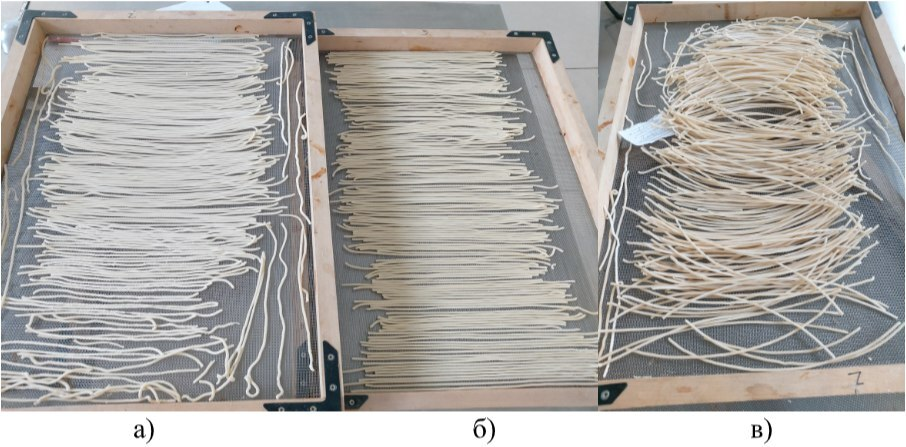
\includegraphics[width=0.6\textwidth]{assets/317-7}
	\caption*{\emph{а) макаронное изделие с тонкодисперсным порошком из гречихи; б)
  макаронное изделие с тонкодисперсным порошком из чечевицы; в) макаронное
  изделие с нанокарбоксилатами.}
  
  {Рис. 1 -- Фото обогащенных макаронных изделий в виде лапши}}
\end{figure}



Были получены 3 вида обогащенных макаронных изделий в виде лапши в
соответствии с разработанной рецептурой:

- макаронное изделие с тонкодисперсным порошком из гречихи;

- макаронное изделие с тонкодисперсным порошком из чечевицы;

- макаронное изделие с нанокарбоксилатами.

Результаты химического анализа обогащенных макаронных изделий с
нанокарбоксилатами и тонкодисперсными порошками из гречневой и
чечевичной муки представлены в таблице 4.

{\bfseries Таблица 4 - Химический анализ обогащенных макаронных изделий с
нанокарбоксилатами и тонкодисперсными порошками из гречневой и
чечевичной муки}

\begin{longtable}[]{@{}
  >{\raggedright\arraybackslash}p{(\columnwidth - 12\tabcolsep) * \real{0.3013}}
  >{\raggedright\arraybackslash}p{(\columnwidth - 12\tabcolsep) * \real{0.1270}}
  >{\raggedright\arraybackslash}p{(\columnwidth - 12\tabcolsep) * \real{0.1111}}
  >{\raggedright\arraybackslash}p{(\columnwidth - 12\tabcolsep) * \real{0.1587}}
  >{\raggedright\arraybackslash}p{(\columnwidth - 12\tabcolsep) * \real{0.1112}}
  >{\raggedright\arraybackslash}p{(\columnwidth - 12\tabcolsep) * \real{0.0793}}
  >{\raggedright\arraybackslash}p{(\columnwidth - 12\tabcolsep) * \real{0.1112}}@{}}
\toprule\noalign{}
\multirow{3}{=}{\begin{minipage}[b]{\linewidth}\raggedright
Наименование макаронных изделий
\end{minipage}} &
\multicolumn{6}{>{\raggedright\arraybackslash}p{(\columnwidth - 12\tabcolsep) * \real{0.6987} + 10\tabcolsep}@{}}{%
\begin{minipage}[b]{\linewidth}\raggedright
Химические показатели
\end{minipage}} \\
&
\multicolumn{3}{>{\raggedright\arraybackslash}p{(\columnwidth - 12\tabcolsep) * \real{0.3969} + 4\tabcolsep}}{%
\begin{minipage}[b]{\linewidth}\raggedright
массовая доля, \%
\end{minipage}} &
\multicolumn{3}{>{\raggedright\arraybackslash}p{(\columnwidth - 12\tabcolsep) * \real{0.3018} + 4\tabcolsep}@{}}{%
\begin{minipage}[b]{\linewidth}\raggedright
Микроэлементы
\end{minipage}} \\
& \begin{minipage}[b]{\linewidth}\raggedright
белка
\end{minipage} & \begin{minipage}[b]{\linewidth}\raggedright
клетчатки
\end{minipage} & \begin{minipage}[b]{\linewidth}\raggedright
углевода
\end{minipage} & \begin{minipage}[b]{\linewidth}\raggedright
Mg
\end{minipage} & \begin{minipage}[b]{\linewidth}\raggedright
Zn
\end{minipage} & \begin{minipage}[b]{\linewidth}\raggedright
Se
\end{minipage} \\
\midrule\noalign{}
\endhead
\bottomrule\noalign{}
\endlastfoot
С тонкодисперсным порошком из гречихи & 11,38 & 5,54 & 50,34 & - & - &
- \\
С тонкодисперсным порошком из чечевицы & 12,16 & 3,49 & 54,18 & - & - &
- \\
С нано-карбоксилатами & 9,33 & 2,17 & 53,75 & 36,84 & 0,78 & Не обн. \\
Контрольный образец & 9,31 & 2,16 & 52,4 & - & - & - \\
\end{longtable}

Результаты исследований показали, что обогащение макаронных изделий
тонкодисперсными порошками привели к значительному повышению пищевой
ценности. Так, добавление 10\% тонкодисперсного порошка из чечевицы к
мучной смеси для производства макарон привело к увеличению белка в
готовых изделиях, в сравнении с контрольным образцом, на 2,85\%,
клетчатки -- 1,33\%. Добавление 10\% гречневого тонкодисперсного порошка
увеличило массовую долю белка на 2,07\%, клетчатки -- 3,35\%.

Добавление нанокарбоксилатов магния, цинка и селена показало наличие в
готовых макаронных изделиях только магния и цинка. Отсутствие селена, по
данным исследований, объясняется тем, что и в прежних исследованиях
наблюдались потери селена в процессе помола муки и в технологиях пищевой
промышленности, что и привело к тому, что селен не был обнаружен в
мучной смеси {[}26{]}.

Характеристика полученных макаронных изделий:

- макаронное изделие с тонкодисперсным порошком из гречихи имеет светло
коричневый цвет, запах свойственный данному изделию, без постороннего
запаха, поверхность гладкая;

- макаронное изделие с тонкодисперсным порошком из чечевицы имеет темно
коричневый цвет, запах свойственный данному изделию, без постороннего
запаха, поверхность гладкая;

- макаронное изделие с нанокарбоксилатами имеет светло коричневый цвет,
запах свойственный данному изделию, без постороннего запаха, поверхность
гладкая.

Таким образом, все три варианта обогащения макаронных изделий можно
рекомендовать для производства.

{\bfseries Выводы.} Целями исследований было получение обогащённых
нанокарбоксилатами и тонкодисперсным порошком из зерновых культур
высокой питательной ценности, употребление которых позволило бы
максимально обеспечить суточные потребности в микронутриентах для
сохранения здоровья населения. Полученные в ходе исследований макаронные
изделия соответствовали требуемым потребительским достоинствам и могут
быть рекомендованы для производства.

\emph{{\bfseries Финансирование:} Представленные результаты получены в
рамках грантового финансирования № DP21681826 «Разработка технологии
производства макаронных изделий, обогащенных микроэлементами»}



\begin{center}
  {\bfseries Литература}
  \end{center}

\begin{noparindent}

1. Любимая лапша: потребление макаронных изделий в Казахстане --- одно
из самых высоких в мире, РК уступает в этом разве что Италии. -URL:
https://finprom.kz/ru/article/lyubimaya-lapsha-potreblenie-makaronnyh-izdelij-v-kazahstane-odno-iz-samyh-vysokih-v-mire-rk-ustupaet-v-etom-razve-chto-italii
\\{[}Дата обращения 27.05.2024{]}

2. Sissons M. Pasta. In: Wrigley C., Corke H., Seetharaman K., Faubion
J., editors. Encyclopedia of Food Grains. 2nd ed. -- Oxford: Academic
Press, 2016. - P. 79--89. {[}Google Scholar{]}

3. Bustos M.C., Perez G.T., Leon A.E. Structure and quality of pasta
enriched with functional ingredients // RSC Adv. -- 2015. --Vol. 5.
-P.30780--30792. DOI: 10.1039/C4RA11857J.

4. Mercier S., Moresoli C., Mondor M., Villeneuve S., Marcos B. A
Meta-analysis of enriched pasta: What are the effects of enrichment and
process specifications on the quality attributes of pasta? Compr. Rev.
Food Sci. Food Saf. 2016;15:685--704. DOI: 10.1111/1541-4337.12207.

5. ГОСТ 31743---2017 «Изделия макаронные. Общие технические условия».
--Москва, Москва \\Стандартинформ, 2017. -9 с.6. ГОСТ 2874-82 «Вода
питьевая. Гигиенические требования и контроль за качеством». - ИПК
издательство стандартов Москва, 1997.

7. Wahanik A.L., Chang Y.K., Clerici P.S., Teresa M. How to make pastas
healthier? // Food Rev. Int. -- 2018. --Vol. (34). --P. 23--30. DOI:
10.1080/87559129.2016.1210634,

8. Li M., Zhu K.-X., Guo X.-N., Brijs K., Zhou H.-M. Natural additives
in wheat-based pasta and noodle products: Opportunities for enhanced
nutritional and functional properties //Compr. Rev. Food Sci. Food Saf.
-- 2014. --Vol.13(4). --P. 347--357. DOI: 10.1111/1541-4337.12066

9. Mike Sissons Development of novel pasta products with evidence based
impacts on health---a review. -2022. --Vol. 11(1). DOI:
10.3390/foods11010123

10. Dariusz Dziki. Current Trends in Enrichment of Wheat Pasta: Quality,
Nutritional Value and Antioxidant Properties. -- 2021. -Vol.9(8).
DOI:10.3390/pr9081280

11. Арсеньева, Л.Ю., Борисенко, О.В., Доценко, В.Ф. Теоретические и
практические аспекты \\использования тонкодиспергованых концентратов
пищевых волокон в технологи ржано-пшеничного хлеба // Научные работы
НУПТ. -2008. -№25. -- C. 115-119.

12. Anthony J. Hennessy J., Andrew R. Davies Disorders of Trace Elements
and Vitamins// Critical Care Nephrology (Second Edition). - 2009. --P.
540-545. DOI:10.1016/B978-1-4160-4252-5.50106-4

13. Скальный А. Микроэлементы: бодрость, здоровье, долголетие. Изд. 4-е,
дополненное, \\переработанное. --М.: Изд-во «Перо», 2019. -295 с. ISBN
978-5-00150-066-7

14. Micronutrient Deficiency. Hannah Ritchie, Max Roser. --URL:
https://ourworldindata.org/micronutrient-deficiency. {[}date of the
application 26.01.2023{]}

15. Hanife Akça and Süleyman Taban Biofortification: zinc enrichment
strategies in crops // Modern Concepts \& Developments in Agronomy.
Submission: -2021. --P. 778-782. \\DOI: 10.31031/MCDA.2021.08.000679

16. S Y Yu 1, Y J Zhu, W G Li Protective role of selenium against
hepatitis B virus and primary liver cancer in Qidong //Biological Trace
Element Research. 1997. --Vol. 56(1). --P. 117-124. DOI:
10.1007/BF02778987.

17. Kieliszek M, Błażejak S. Current Knowledge on the Importance of
Selenium in Food for Living Organisms: A Review // Molecules. -20167
--Vol. 21(5). DOI: 10.3390/molecules21050609

18. Aparna P. Shreenath; Muhammad Atif Ameer; Jennifer Dooley Selenium
Deficiency: StatPearls --URL:
https://www.ncbi.nlm.nih.gov/books/NBK482260/ {[}date of the application
03.06.2024{]}

19. Viering D. H. H. M., de Baaij J. H. F., Walsh S. B., Kleta R.,
Bockenhauer D. Genetic causes of hypomagnesemia, a clinical overview //
Pediatric Nephrology. -2017. --Vol. 32(7). --P. 1123--1135. DOI:
10.1007/s00467-016-3416-3

20. Abdullah M. Al Alawi, Sandawana William Majoni and Henrik Falhammar
Magnesium and Human Health: Perspectives and Research Directions //
International Journal of Endocrinology. -- 2018. DOI:
10.1155/2018/9041694

21. Costello RB, Elin RJ, Rosanoff A, et al.. Perspective: the case for
an evidence-based reference interval for serum magnesium: The time has
come // Advances in Nutrition: An International Review. -2016.
--Vol.7(6). --P. 977--993. DOI: 10.3945/an.116.012765

22. Philip G Crandall, Han-Seok Seo, Corliss A O\textquotesingle Bryan,
Jf C Meullenet. Physicochemical analysis of wheat flour fortified with
vitamin A and three types of iron source and sensory analysis of bread
using these flours// Journal of the Science of Food and Agriculture.
-2013. --Vol. 93(9). --P. 2299-2307. \\DOI:10.1002/jsfa.6043

23. .Shaimerdenova D.A., Chakanova Z.M., Sultanova M.Z., Shaimerdenova
P.R., Abdrakhmanov K.A. Instant cereals enriched with
carboxylatesInternational // Journal of Engineering and Technology(UAE).
-- 2018. --Vol. 7(2). --P. 140--144

24. Приказ Министра национальной экономики Республики Казахстан от 9
декабря 2016 года № 503 «Об утверждении научно обоснованных
физиологических норм потребления продуктов питания» // Министерство
юстиции Республики Казахстан. -2016.

25. Annalisa Romano, Veronica Gallo, Pasquale Ferranti. Paolo Masi
Lentil flour: nutritional and \\technological properties, in vitro
digestibility and perspectives for use in the food industry // Current
Opinion in Food Science. -2021. --Vol. 40. --P. 157-167. DOI:
10.1016/j.cofs.2021.04.003

26. Min Wang, Baoqiang Li, Shuang Li, Ziwei Song, Fanmei Kong, Xiaocun
Zhang Selenium in wheat from farming to food // Journal of Agricultural
and Food Chemistry. -- 2021. --Vol. 69. --P. 15458--15467. DOI:
10.1101/2021.07.17.452805.

\end{noparindent}

\begin{center}
{\bfseries References}
\end{center}

\begin{noparindent}

1. Lyubimaya lapsha: potreblenie makaronnykh izdelii v Kazakhstane ---
odno iz samykh vysokikh v mire, RK ustupaet v etom razve chto Italii.
-URL:
https://finprom.kz/ru/article/lyubimaya-lapsha-potreblenie-makaronnyh-izdelij-v-kazahstane-odno-iz-samyh-vysokih-v-mire-rk-ustupaet-v-etom-razve-chto-italii
\\(Data obrashcheniya 27.05.2024) {[}in Russian{]}

2. Sissons M. Pasta. In: Wrigley C., Corke H., Seetharaman K., Faubion
J., editors. Encyclopedia of Food Grains. 2nd ed. -- Oxford: Academic
Press, 2016. - P. 79--89. {[}Google Scholar{]}

3. Bustos M.C., Perez G.T., Leon A.E. Structure and quality of pasta
enriched with functional ingredients // RSC Adv. -- 2015. --Vol. 5.
-P.30780--30792. DOI: 10.1039/C4RA11857J.

4. Mercier S., Moresoli C., Mondor M., Villeneuve S., Marcos B. A
Meta-analysis of enriched pasta: What are the effects of enrichment and
process specifications on the quality attributes of pasta? Compr. Rev.
Food Sci. Food Saf. 2016;15:685--704. DOI: 10.1111/1541-4337.12207.

5. GOST 31743---2017 «Izdeliya makaronnye. Obshchie tekhnicheskie
usloviya». --Moskva, Moskva \\Standartinform, 2017. -9 s. 6. GOST 2874-82
«Voda pit\textquotesingle evaya. Gigienicheskie trebovaniya i
kontrol\textquotesingle{} za kachestvom». - IPK
izdatel\textquotesingle stvo standartov Moskva, 1997. {[}in Russian{]}

7. Wahanik A.L., Chang Y.K., Clerici P.S., Teresa M. How to make pastas
healthier? // Food Rev. Int. -- 2018. --Vol. (34). --P. 23--30. DOI:
10.1080/87559129.2016.1210634,

8. Li M., Zhu K.-X., Guo X.-N., Brijs K., Zhou H.-M. Natural additives
in wheat-based pasta and noodle products: Opportunities for enhanced
nutritional and functional properties //Compr. Rev. Food Sci. Food Saf.
-- 2014. --Vol.13(4). --P. 347--357. DOI: 10.1111/1541-4337.12066

9. Mike Sissons Development of novel pasta products with evidence based
impacts on health---a review. -2022. --Vol. 11(1). DOI:
10.3390/foods11010123

10. Dariusz Dziki. Current Trends in Enrichment of Wheat Pasta: Quality,
Nutritional Value and Antioxidant Properties. -- 2021. -Vol.9(8).
DOI:10.3390/pr9081280

11. Arsen\textquotesingle eva, L.Yu., Borisenko, O.V., Dotsenko, V.F.
Teoreticheskie i prakticheskie aspekty ispol\textquotesingle zovaniya
tonkodispergovanykh kontsentratov pishchevykh volokon v tekhnologi
rzhano-pshenichnogo khleba // Nauchnye raboty NUPT. -2008. -№25. -- C.
115-119. {[}in Russian{]}

12. Anthony J. Hennessy J., Andrew R. Davies Disorders of Trace Elements
and Vitamins// Critical Care Nephrology (Second Edition). - 2009. --P.
540-545. DOI:10.1016/B978-1-4160-4252-5.50106-4

13. Skal\textquotesingle nyi A. Mikroelementy: bodrost\textquotesingle,
zdorov\textquotesingle e, dolgoletie. Izd. 4-e, dopolnennoe,
pererabotannoe. --M.: Izd-vo «Pero», 2019. -295 s. ISBN
978-5-00150-066-7 {[}in Russian{]}

14. Micronutrient Deficiency. Hannah Ritchie, Max Roser. --URL:
https://ourworldindata.org/micronutrient-deficiency. {[}date of the
application 26.01.2023{]}

15. Hanife Akça and Süleyman Taban Biofortification: zinc enrichment
strategies in crops // Modern Concepts \& Developments in Agronomy.
Submission: -2021. --P. 778-782.\\ DOI: 10.31031/MCDA.2021.08.000679

16. S Y Yu 1, Y J Zhu, W G Li Protective role of selenium against
hepatitis B virus and primary liver cancer in Qidong //Biological Trace
Element Research. 1997. --Vol. 56(1). --P. 117-124. DOI:
10.1007/BF02778987.

17. Kieliszek M, Błażejak S. Current Knowledge on the Importance of
Selenium in Food for Living Organisms: A Review // Molecules. -20167
--Vol. 21(5). DOI: 10.3390/molecules21050609

18. Aparna P. Shreenath; Muhammad Atif Ameer; Jennifer Dooley Selenium
Deficiency: StatPearls --URL:
https://www.ncbi.nlm.nih.gov/books/NBK482260/ {[}date of the application
03.06.2024{]}

19. Viering D. H. H. M., de Baaij J. H. F., Walsh S. B., Kleta R.,
Bockenhauer D. Genetic causes of hypomagnesemia, a clinical overview //
Pediatric Nephrology. -2017. --Vol. 32(7). --P. 1123--1135. DOI:
10.1007/s00467-016-3416-3

20. Abdullah M. Al Alawi, Sandawana William Majoni and Henrik Falhammar
Magnesium and Human Health: Perspectives and Research Directions //
International Journal of Endocrinology. -- 2018. DOI:
10.1155/2018/9041694

21. Costello RB, Elin RJ, Rosanoff A, et al.. Perspective: the case for
an evidence-based reference interval for serum magnesium: The time has
come // Advances in Nutrition: An International Review. -2016.
--Vol.7(6). --P. 977--993. DOI: 10.3945/an.116.012765

22. Philip G Crandall, Han-Seok Seo, Corliss A O\textquotesingle Bryan,
Jf C Meullenet. Physicochemical analysis of wheat flour fortified with
vitamin A and three types of iron source and sensory analysis of bread
using these flours// Journal of the Science of Food and Agriculture.
-2013. --Vol. 93(9). --P. 2299-2307. \\DOI:10.1002/jsfa.6043

23. .Shaimerdenova D.A., Chakanova Z.M., Sultanova M.Z., Shaimerdenova
P.R., Abdrakhmanov K.A. Instant cereals enriched with
carboxylatesInternational // Journal of Engineering and Technology(UAE).
-- 2018. --Vol. 7(2). --P. 140--144

24. Prikaz Ministra natsional\textquotesingle noi ekonomiki Respubliki
Kazakhstan ot 9 dekabrya 2016 goda № 503 «Ob utverzhdenii nauchno
obosnovannykh fiziologicheskikh norm potrebleniya produktov pitaniya» //
Ministerstvo yustitsii Respubliki Kazakhstan. -2016. {[}in Russian{]}

25. Annalisa Romano, Veronica Gallo, Pasquale Ferranti. Paolo Masi
Lentil flour: nutritional and \\technological properties, in vitro
digestibility and perspectives for use in the food industry // Current
Opinion in Food Science. -2021. --Vol. 40. --P. 157-167. DOI:
10.1016/j.cofs.2021.04.003

26. Min Wang, Baoqiang Li, Shuang Li, Ziwei Song, Fanmei Kong, Xiaocun
Zhang Selenium in wheat from farming to food // Journal of Agricultural
and Food Chemistry. -- 2021. --Vol. 69. --P. 15458--15467. DOI:
10.1101/2021.07.17.452805.

\end{noparindent}

\emph{{\bfseries Сведения об авторах}}

\begin{noparindent}

Шаймерденова Д.А. - доктор технических наук, ТОО
"Научно-производственное предприятие \\"Инноватор", Астана, Казахстан,
e-mail: darigash@mail.ru;

Омаралиева А.М. - кандидат технических наук, ассоциированный профессор
кафедры «Технология и стандартизация», АО «Казахский университет
технологии и бизнеса» им. К. Кулажанова» Астана, Казахстан, e-mail:
aigul-omar@mail.ru;

Тарабаев Б.К. - кандидат технических наук, «Казахский агротехнический
исследовательский универ-ситет. Сейфуллин", Астана, Казахстан,
e-mail:tarabaev50@mail.ru;

Сарбасова Л.Т. - кандидат технических наук, ТОО "Научно-производственное
предприятие \\"Инноватор", Астана, Казахстан, e-mail: sargt@mail.ru;

Ануарбекова С.С. -- кандидат медицинских наук, ТОО
"Научно-производственное предприятие \\"Инноватор", Астана, Казахстан,
e-mail: sanuarbekova@rambler.ru;

Искакова Д.Б. - ТОО "Научно-производственное предприятие "Инноватор ",
Астана, Казахстан, e-mail: damirais 61@mail.ru;

Шаймерденов А.А. - ТОО ``Научно-производственное предприятие ``Инноватор
``, Астана, Казахстан, e-mail: darigash@mail.ru;

Тастанов Д.А. - ТОО ``Научно-производственное предприятие ``Инноватор
``, Астана, Казахстан,e-mail: dias.tastanov@mail.ru

\end{noparindent}

\emph{{\bfseries Information about authors}}

\begin{noparindent}

Shaimerdenova D. A. - Doctor of Technical Sciences, «Scientific and
production enterprise «Innovator» LLP, Astana, Kazakhstan, e-mail:
darigash@mail.ru;

Omaralieva A. M. - Candidate of Technical Sciences, Associate Professor
of the Department of Technology and Standardization of "K. Kulazhanov
Kazakh University of Technology and Business JSC" Astana, е-mail:
aigul-omar@mail.ru;

Tarabayev B.K. - Candidate of Technical Sciences, Kazakh Agrotechnical
Research University Seifullin, Astana, Kazakhstan, e-mail:
tarabaev50@mail.ru;

Sarbasova L.T. - Candidate of Technical Sciences, «Scientific and
production enterprise «Innovator» LLP, ,Astana, Kazakhstan, e-mail:
sargt@mail.ru;

Anuarbekova S.S. - Candidate of Medical Sciences, «Scientific and
production enterprise «Innovator» LLP, , Astana, Kazakhstan, e-mail:
sanuarbekova@rambler.ru;

Iskakova D.B. -«Scientific and production enterprise «Innovator» LLP,
Astana, Kazakhstan,\\e-mail: damirais 61@mail.ru;

Shaimerdenov A.A. - Scientific and Production Enterprise «Innovator»
LLP, Kazakhstan, Astana, LLP «Scientific and production enterprise
«Innovator», Astana, Kazakhstan, e-mail: darigash@mail.ru;

Tastanov D.A. - «Scientific and production enterprise «Innovator» LLP,
Astana, Kazakhstan, e-mail: dias.tastanov@mail.ru


\end{noparindent}







